

    The DAGA cothority was simulated both locally and on DETERLab facilities using the simulation tools provided by Onet.\sidecite{dedis_cothority_nodate}
    The local simulations were run on a 64-bit x86 machine running Debian 9\sidenote{
        CPU: 8 * i7-4710HQ @ 2.50GHz
        RAM: 16GiB
    }
    The DETERLab simulations were run with \emph{pc2133} nodes\sidenote{
        CPU: 4 * Xeon-X3210 @ 2.13GHz
        RAM: 4GiB
    } running Ubuntu 14.04 and connected to the same LAN,  where a delay of 100ms was added between each nodes.

    As was done in the previous works\cite{syta_identity_2015,villard_report_pfs_pop.pdf_2017} we varied the number of clients from
    2 to 32768 by power of 2 and repeated the experiment for cothorities of size 2,4,8,16 and 32.

    As a key difference to the simulations performed by~\cite{syta_identity_2015} and~\cite{villard_report_pfs_pop.pdf_2017}
    the simulations that were performed here are featuring real network communications between different (remote) processes.\sidenote{
        even for the local simulations, all conodes are living in their onw process and all communications are going through the network stack
    }

    \subsection{Authentication time}
    \label{subsec:test123}
    Fig.~\ref{fig:authtime} % FIXME RHAAAAAAAAAAAAAAAAAAAAAA F/*%@# latex wrong fig number !!!!!!!!
    %The following figure
    shows the total wall time needed to authenticate with the cothority.\sidenote{
        PKClient included, i.e.\ from the start of the client protocol until the final tag is received.
    }\vspace*{1cm}
%    \begin{figure*}
%        \centering
%        \subfigure[deterlab simulation]{
%            \centering
%            \caption{auth.\ time on deterlab}
%            \label{fig:deterlabauthtime}
%            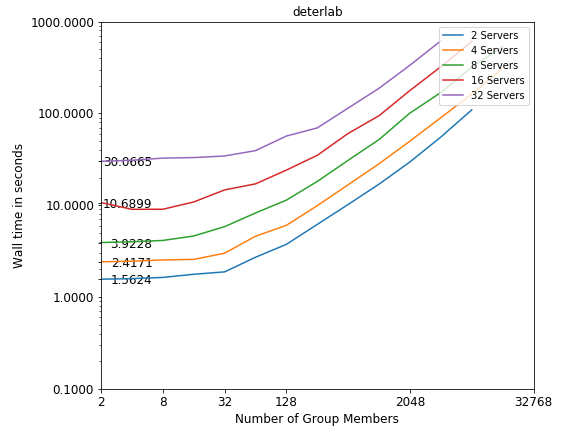
\includegraphics[width=.4\linewidth]{images/plots/authwalltime_deterlab.png} % svg gives me an error
%        }
%        \subfigure[local simulation]{
%            \centering
%            \caption{auth.\ time locally}
%            \label{fig:localauthtime}
%            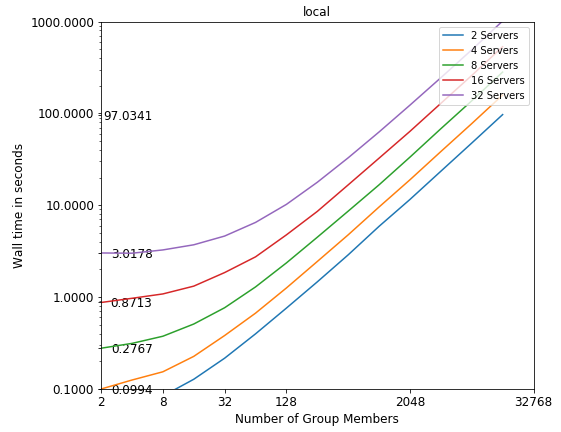
\includegraphics[width=.4\linewidth]{images/plots/authwalltime_local.png}
%        }

%        \begin{subfigure}
%           \centering
%%            \caption{auth.\ time locally}
%%            \label{fig:localauthtime}
%           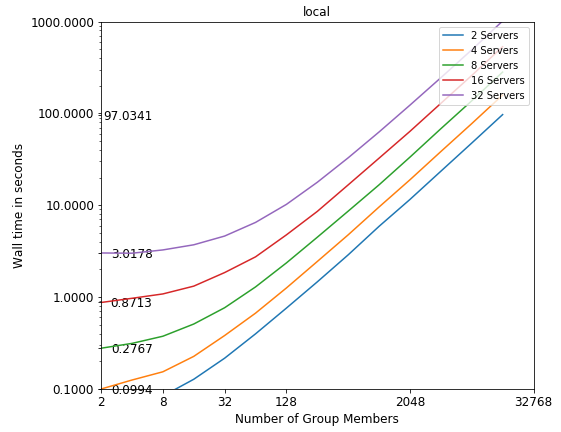
\includegraphics[width=.4\linewidth]{images/plots/authwalltime_local.png}
%        \end{subfigure}
%        \begin{subfigure}
%            \centering
%%            \caption{auth.\ time locally}
%%            \label{fig:localauthtime}
%            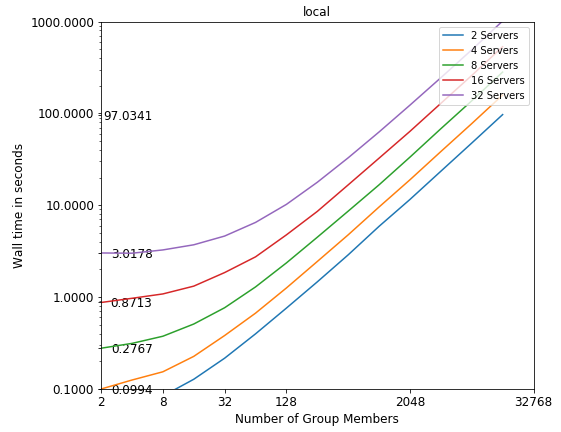
\includegraphics[width=.4\linewidth]{images/plots/authwalltime_local.png}
%        \end{subfigure}
    \begin{figure*}
        \centering
        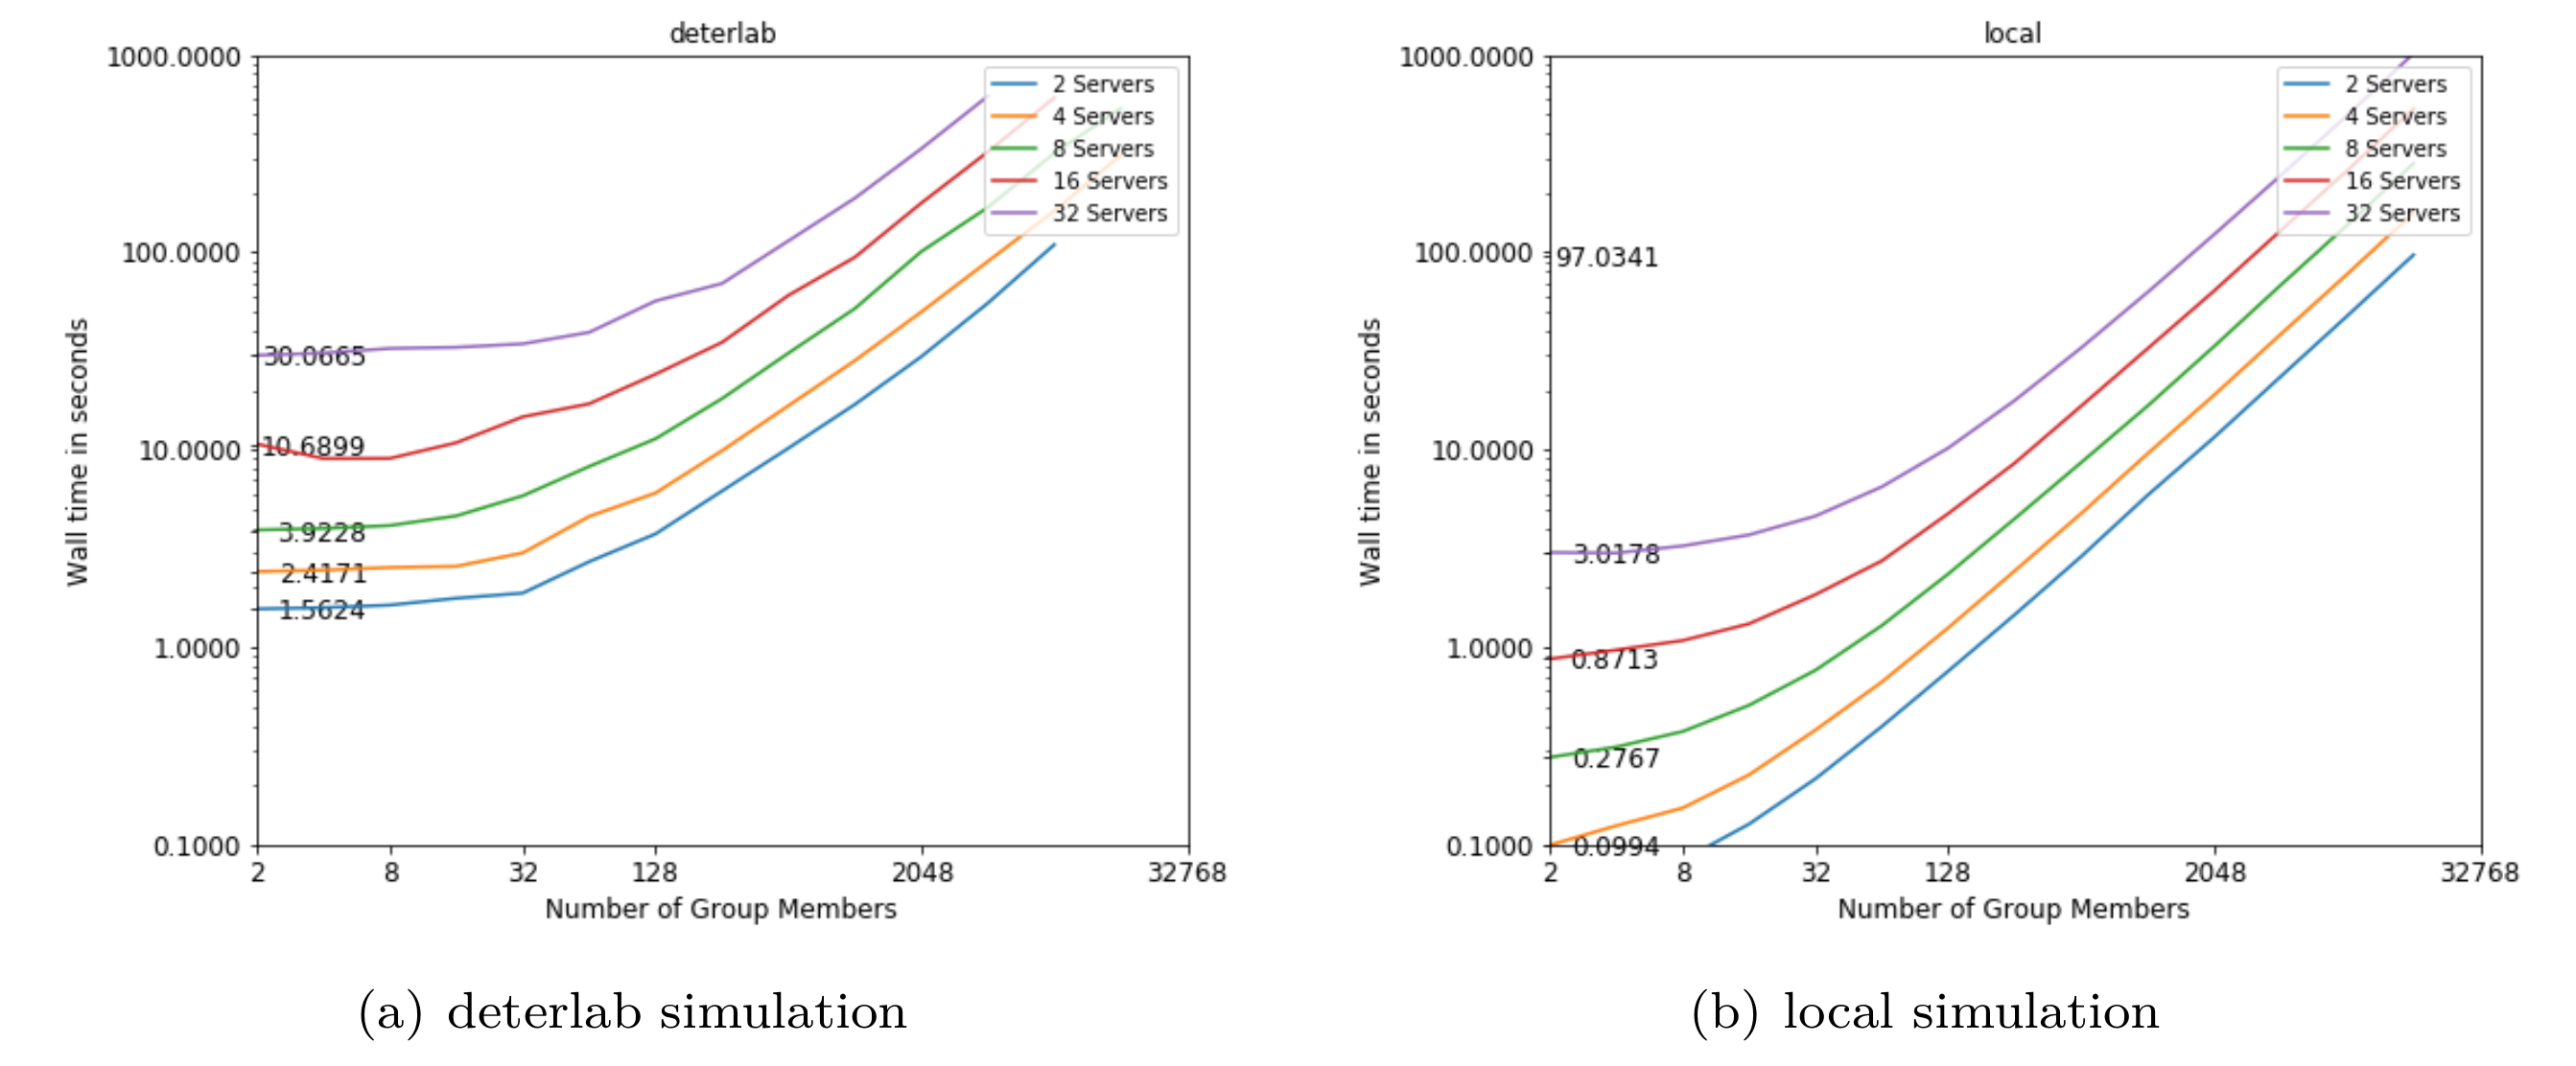
\includegraphics[width=0.8\linewidth]{images/plots/authenticationtimeHack.png}
        \vspace*{1cm}
        \caption{Authentication wall time}
        \label{fig:authtime}
    \end{figure*}
    We can clearly observe the impact of the 100ms delay existing in the DETERLab setting.
    Comparing the results of the local simulation with the one of~\cite{villard_report_pfs_pop.pdf_2017} we can observe
    a small overhead, probably because now we are running a real cothority (overhead of the cothority framework and network communication).
    Hence in all logic when comparing it to the one of~\cite{syta_identity_2015} we notice improvements of the same order
    as the one noticed in~\cite{villard_report_pfs_pop.pdf_2017}.\sidenote{(~10X) for the same reasons, notably moore's law}
    We can see that even when running our simulation in a real world setting (DETERLab) with network delays, we obtain
    authentication times comparable to or only slightly slower than the ones obtained by~\cite{syta_identity_2015}

    \subsubsection{PKClient, Auth, and Total time}

    Fig.~\ref{fig:stackedauthtime}  % FIXME RHAAAAAAAAAAAAAAAAAAAAAA F/*%@# latex wrong fig number !!!!!!!!
    %The following figure
    decompose the total authentication wall time\sidenote{
        Only local simulation shown, in deterlab similar with only difference being that at beginning the 100ms delay dominate
        before becoming insignificant later, same difference as in Fig.~\ref{fig:authtime} above.
    } into the time needed to build the proof (blue) and
    the time needed to process the request (orange).\vspace*{0.3cm}
    \begin{figure*}
        \centering
%        \subfigure[2 servers]{
%            \centering
%            \label{fig:stackedlocal2}
%            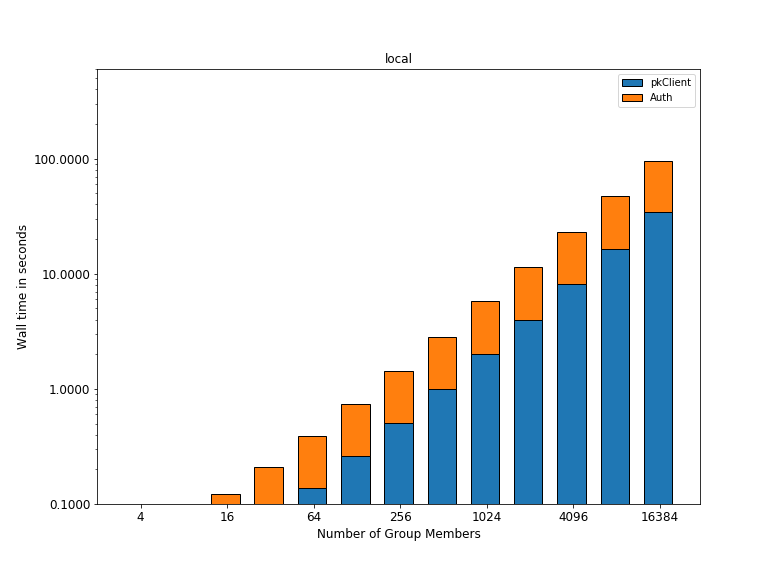
\includegraphics[width=.4\linewidth]{images/plots/stacked2servers_local.png} % svg gives me an error
%        }
%        \subfigure[4 servers]{
%            \centering
%            \label{fig:stackedlocal4}
%            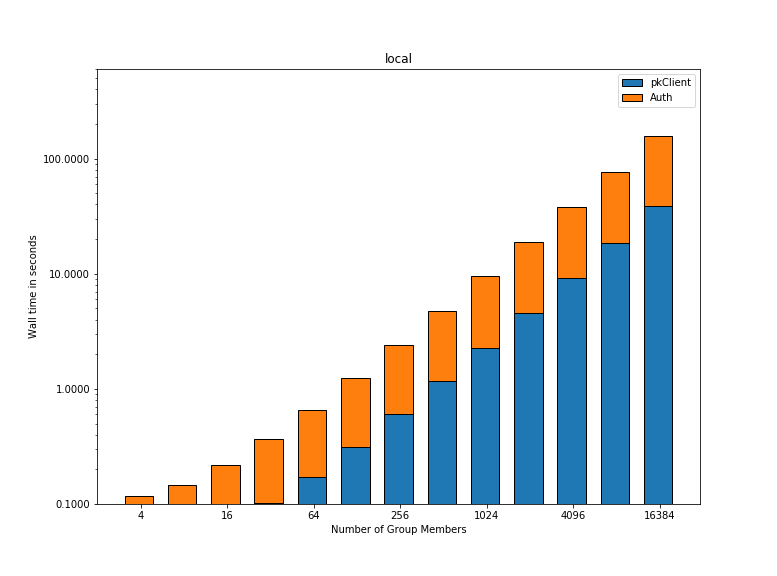
\includegraphics[width=.4\linewidth]{images/plots/stacked4servers_local.png} % svg gives me an error
%        }
%        \subfigure[8 servers]{
%            \centering
%            \label{fig:stackedlocal8}
%            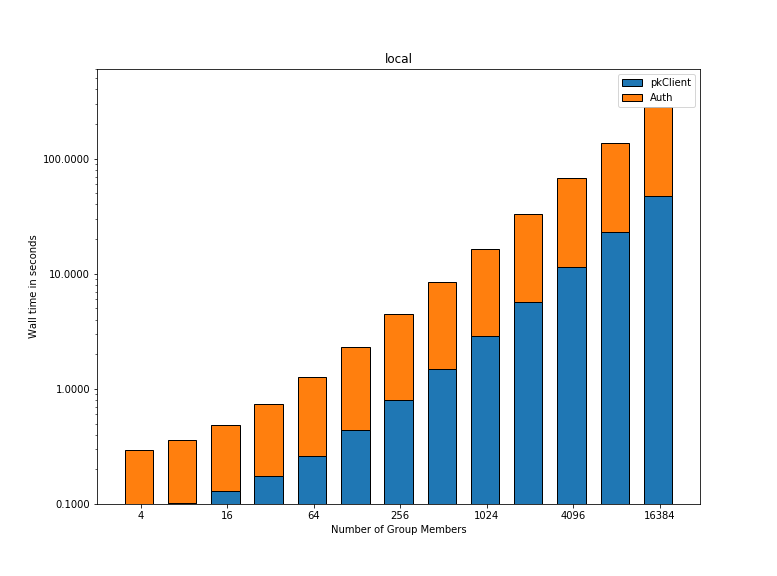
\includegraphics[width=.4\linewidth]{images/plots/stacked8servers_local.png} % svg gives me an error
%        }\newline
%        \subfigure[16 servers]{
%            \centering
%            \label{fig:stackedlocal16}
%            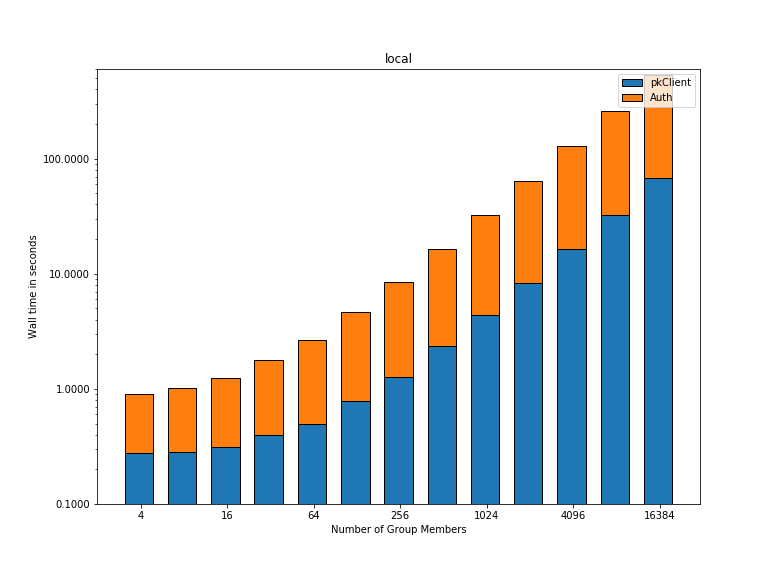
\includegraphics[width=.4\linewidth]{images/plots/stacked16servers_local.png} % svg gives me an error
%        }
%        \subfigure[32 servers]{
%            \centering
%            \label{fig:stackedlocal32}
%            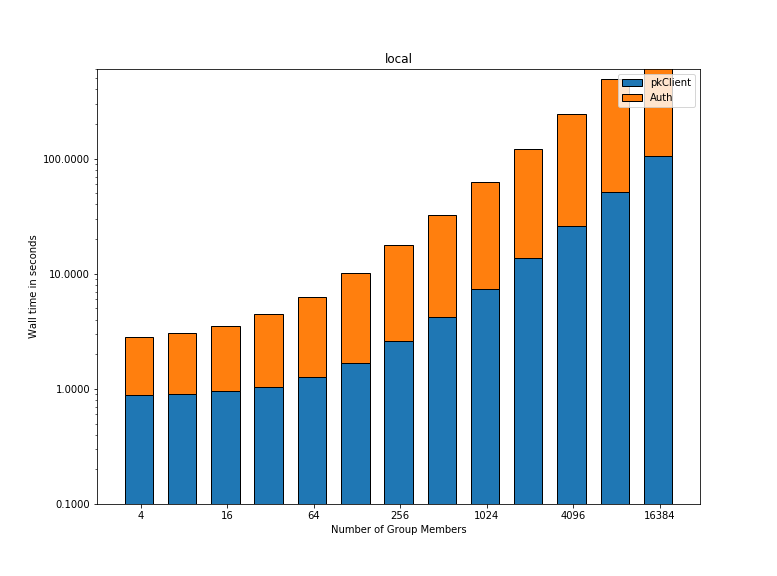
\includegraphics[width=.4\linewidth]{images/plots/stacked32servers_local.png} % svg gives me an error
%        }
        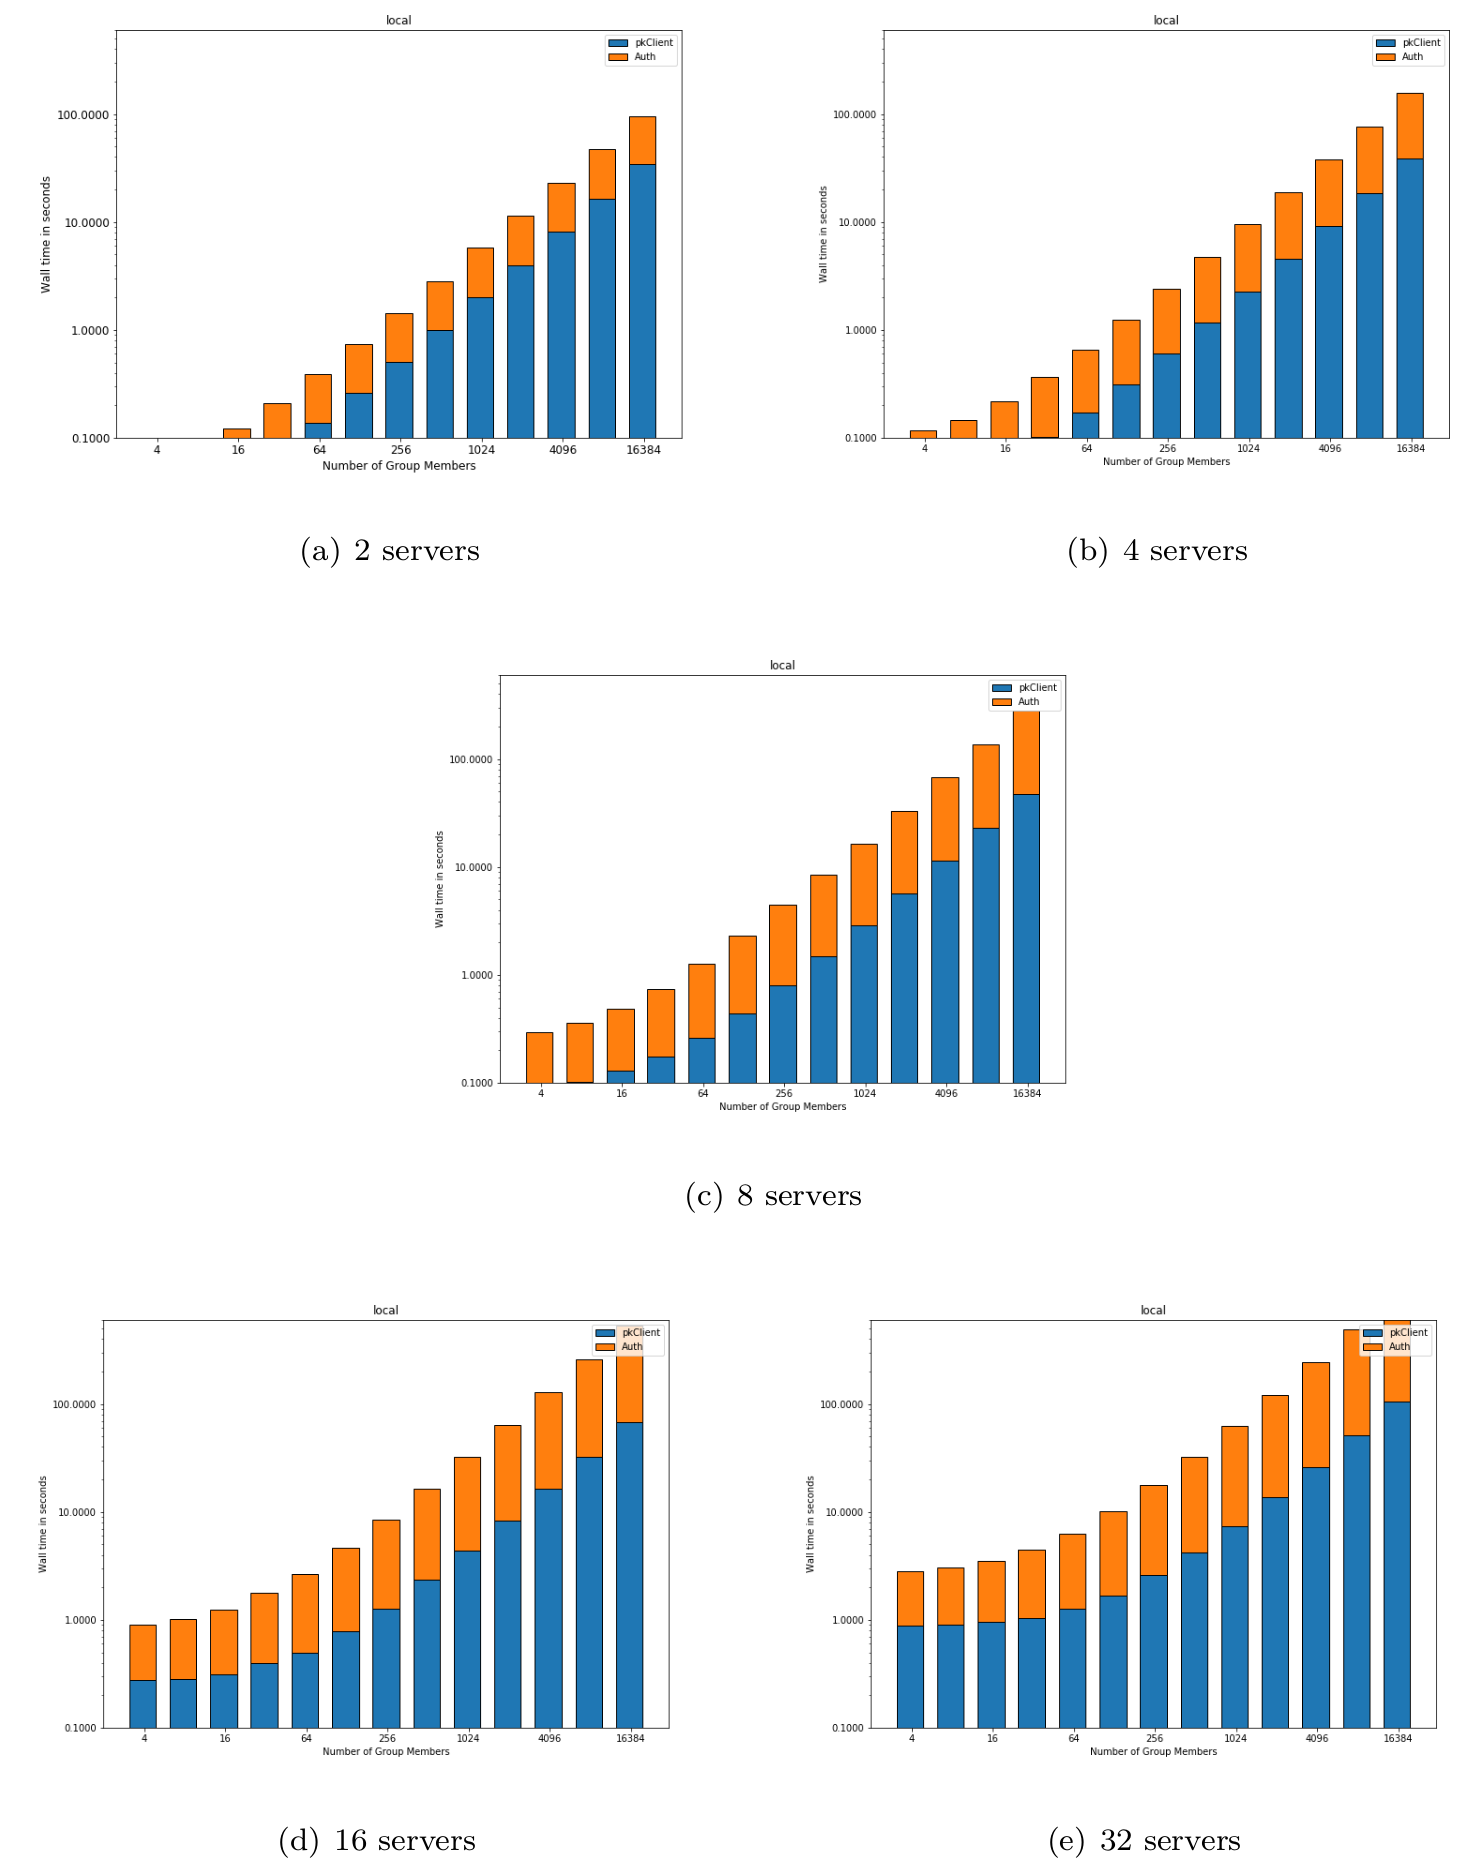
\includegraphics[width=0.8\linewidth]{images/plots/stackedHack.png}
        \vspace*{1cm}
        \caption{Authentication time decomposed}
        \label{fig:stackedauthtime}
    \end{figure*}

    \subsection{Traffic}

    Only the total\sidenote{
        the client-server or server-client traffic should not change much in comparison with~\cite{villard_report_pfs_pop.pdf_2017}.
    } Server traffic was plotted.

    Fig.~\ref{fig:servertraffic} % FIXME RHAAAAAAAAAAAAAAAAAAAAAA F/*%@# latex wrong fig number !!!!!!!!
    %The following figure
    shows the sum of the data sent by each server during the Authentication of a user.

    \begin{figure}
        \centering
        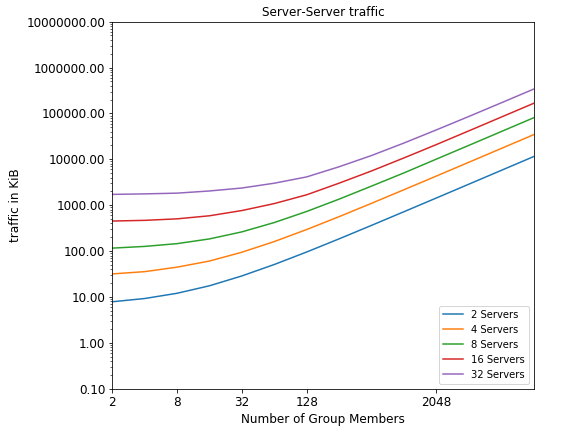
\includegraphics[width=.65\linewidth]{images/plots/serverservertraffic.png} % svg gives me an error
        \vspace*{1cm}
        \caption{Total Server traffic}
        \label{fig:servertraffic}
    \end{figure}

    Finally we share the conclusions that \blockquote{
        all forms of DAGA traffic grow linearly in the number of clients and nearly linearly in the number of servers
    }\cite{syta_identity_2015} hence our results are coherent.

    %TODO ?
    %You can note that there are some holes in the data, that is because we
    % problems : read tcp io timeout, out of memory, ssh keepalive, bug in cothority/onet cache clean/timeout while protocol alive .. ...
    % etc.. etc.. ran short of time and patience


    %the graphs and quick discussion,
    %comment on moore law,
    %say that probably could/should be quicker if X25519 was used (hypothesis, don't make a fool of myself if it is the case)
    %say there are lots of redundant and probably not useful signatures that slowdown everything
    %+ say that coherent with previous implementations